%%% ====================================================================
%%% @LaTeX-file{
%%%   filename  = "aomsample.tex",
%%%   copyright = "Copyright 1995, 1999 American Mathematical Society,
%%%                2005 Hebrew University Magnes Press,
%%%                all rights reserved.  Copying of this file is
%%%                authorized only if either:
%%%                (1) you make absolutely no changes to your copy,
%%%                including name; OR
%%%                (2) if you do make changes, you first rename it
%%%                to some other name.",
%%% }
%%% ====================================================================
\NeedsTeXFormat{LaTeX2e}% LaTeX 2.09 can't be used (nor non-LaTeX)
[1994/12/01]% LaTeX date must December 1994 or later
\documentclass[final]{aomart}
\usepackage[english]{babel}

\usepackage{mathtools,amssymb,amsthm}
\usepackage{bm}
\usepackage{float}

%    Some definitions useful in producing this sort of documentation:
\chardef\bslash=`\\ % p. 424, TeXbook
%    Normalized (nonbold, nonitalic) tt font, to avoid font
%    substitution warning messages if tt is used inside section
%    headings and other places where odd font combinations might
%    result.
\newcommand{\ntt}{\normalfont\ttfamily}
%    command name
\newcommand{\cn}[1]{{\protect\ntt\bslash#1}}
%    LaTeX package name
\newcommand{\pkg}[1]{{\protect\ntt#1}}
%    File name
\newcommand{\fn}[1]{{\protect\ntt#1}}
%    environment name
\newcommand{\env}[1]{{\protect\ntt#1}}
\hfuzz1pc % Don't bother to report overfull boxes if overage is < 1pc

%       Theorem environments

%% \theoremstyle{plain} %% This is the default
\newtheorem[{}\it]{thm}{Theorem}[section]
\newtheorem{cor}[thm]{Corollary}
\newtheorem{lem}[thm]{Lemma}
\newtheorem{prop}[thm]{Property}
\newtheorem{propo}[thm]{Proposition}
\newtheorem{ax}{Axiom}

\theoremstyle{definition}
\newtheorem{defn}{Definition}[section]
\newtheorem{rem}{Remark}[section]
\newtheorem*[{}\it]{notation}{Notation}
\newtheorem{step}{Step}

\numberwithin{equation}{section}

\newcommand{\thmref}[1]{Theorem~\ref{#1}}
\newcommand{\secref}[1]{\S\ref{#1}}
\newcommand{\lemref}[1]{Lemma~\ref{#1}}


%       Math definitions

\newcommand{\A}{\mathcal{A}}
\newcommand{\B}{\mathcal{B}}
\newcommand{\st}{\sigma}
\newcommand{\XcY}{{(X,Y)}}
\newcommand{\SX}{{S_X}}
\newcommand{\SY}{{S_Y}}
\newcommand{\SXY}{{S_{X,Y}}}
\newcommand{\SXgYy}{{S_{X|Y}(y)}}
\newcommand{\Cw}[1]{{\hat C_#1(X|Y)}}
\newcommand{\G}{{G(X|Y)}}
\newcommand{\PY}{{P_{\mathcal{Y}}}}
\newcommand{\X}{\mathcal{X}}
\newcommand{\wt}{\widetilde}
\newcommand{\wh}{\widehat}


\newcommand{\like}{\mathcal{L}} % likelihood
\newcommand{\loglike}{\ell} % log-likelihood
\newcommand{\e}{\mathrm{e}} % euler's constant
\newcommand{\pdf}{f} % probability density function
\newcommand{\htheta}{\hat{\theta}} % estimator (abuse of notation)
\newcommand{\hTheta}{\wh{\Theta}} % estimator
\DeclareMathOperator{\newdiff}{d} % use \dif instead
\newcommand{\dif}{\newdiff\!} % differential operator
\newcommand{\fisher}{\mathcal{I}} % fisher information matrix
\DeclareMathOperator{\var}{var}
\DeclareMathOperator{\cov}{cov}
\DeclareMathOperator{\dom}{dom}
\DeclareMathOperator{\argmax}{arg\,max}
\DeclareMathOperator{\plim}{plim}

\makeatletter
\DeclareRobustCommand{\expe}{\mathbb{E}\@ifstar\@firstofone\@expe}
\newcommand{\@expe}[1]{\left[#1\right]}
\makeatother

\makeatletter
\DeclareRobustCommand{\var}{\mathbb{V}\@ifstar\@firstofone\@expe}
\newcommand{\@var}[1]{\left[#1\right]}
\makeatother

%    \interval is used to provide better spacing after a [ that
%    is used as a closing delimiter.
\newcommand{\interval}[1]{\mathinner{#1}}

%    Notation for an expression evaluated at a particular condition. The
%    optional argument can be used to override automatic sizing of the
%    right vert bar, e.g. \eval[\biggr]{...}_{...}
\newcommand{\eval}[2][\right]{\relax
  \ifx#1\right\relax \left.\fi#2#1\rvert}

%    Enclose the argument in vert-bar delimiters:
\newcommand{\envert}[1]{\left\lvert#1\right\rvert}
\let\abs=\envert

%    Enclose the argument in double-vert-bar delimiters:
\newcommand{\enVert}[1]{\left\lVert#1\right\rVert}
\let\norm=\enVert

%\setcounter{tocdepth}{5}

\title[Fish schools tracking]{LINMA1731 -- Project 2019\\
Fish schools tracking}

\author{Louis Navarre}
\address{Université catholique de Louvain, Ottignies-Louvain-la-Neuve, Belgium}
\fulladdress{École Polytechnique, Université catholique de Louvain, Place de l'Université 1, 1348 Ottignies-Louvain-la-Neuve, Belgique}
\email{navarre.louis@student.uclouvain.be}
\givenname{Louis}
\surname{Navarre}

\author{Gilles Peiffer}
\address{Université catholique de Louvain, Ottignies-Louvain-la-Neuve, Belgium}
\fulladdress{École Polytechnique\\
	Université catholique de Louvain\\
	Place de l'Université 1, 1348 Ottignies-Louvain-la-Neuve, Belgium}
\email{gilles.peiffer@student.uclouvain.be}
\givenname{Gilles}
\surname{Peiffer}

%\oldsubsections
\copyrightnote{\textcopyright~2019 Gilles Peiffer and Louis Navarre}

\begin{document}

\begin{abstract}
	In this paper we solve the first part of the project for the class ``Stochastic processes: Estimation and prediction'' given during the Fall term of 2019.
	The average speed of each fish in a school of fish is approximated by a gamma-distributed random variable with a shape parameter \(k\) and a scale parameter \(s\), and various methods for estimating this quantity are given; a numerical simulation is also included.
\end{abstract}

\maketitle
\tableofcontents

\part{Average speed estimation}
\section{Introduction}
For the purpose of this project, we assume that the speed of each fish in a school
at time \(i\) is a random variable \(V_i\) following a Gamma distribution, as suggested in [1].
This distribution is characterized by two parameters:
a shape parameter \(k > 0\) and a scale parameter \(s > 0\).
The parameters are the same for every fish and are time invariant.
The aim of this first part is to identify these two parameters using empirical observations \(v_i\).

\section{Maximum likelihood estimation}
Let \(v_i\) be i.i.d. realisations of a random variable following a Gamma distribution \(\Gamma(k, s)\) (with \(i = 1,\ldots, N)\).
We first assume that the shape parameter \(k\) is known.

We start by deriving the maximum likelihood estimator of \(\theta \coloneqq s\) based on \(N\) observations.
Since the estimand $\theta$ is a deterministic quantity, we use Fisher estimation.
In order to do this, let us restate the probability density function of \(V_i \sim \Gamma(k, s)\):
\begin{equation}
\pdf_{V_i}(v_i; k, s) = \frac{1}{\Gamma(k) s^k} v_i^{k-1} \e^{-\frac{v_i}{s}}\,, \quad i = 1, \ldots, N\,.
\end{equation}
With this in mind, we can find that the likelihood \(\like(v_1, \ldots, v_N; k, \theta)\) is given by
\begin{align}
\like(v_1, \ldots, v_N; k, \theta) &= \prod_{i=1}^{N} \pdf_{V_i}(v_i; k,\theta) = \prod_{i=1}^{N} \frac{1}{\Gamma(k) \theta^k} v_i^{k-1} \e^{-\frac{v_i}{\theta}}\,.
\end{align}
In order to alleviate notation, we compute instead the log-likelihood, which is generally easier to work with\footnote{This is possible because the values of \(\theta\) which maximize the log-likelihood also maximize the likelihood.}:
\begin{align}
\ell(v_1, \ldots, v_N; k, \theta) &\coloneqq \ln \like(v_1, \ldots, v_N; k, \theta)\\
& = \sum_{i=1}^{N} \ln\Bigg(\frac{1}{\Gamma(k) \theta^k} v_i^{k-1} \e^{-\frac{v_i}{\theta}}\Bigg)\\
& = (k-1) \sum_{i=1}^{N}\ln v_i - \sum_{i=1}^{N} \frac{v_i}{\theta} - N \big(k \ln \theta + \ln \Gamma(k)\big)\,.\label{loglikelihood}
\end{align}
Now, in order to obtain the maximum likelihood estimate \(\htheta\), we must differentiate the log-likelihood with respect to the estimand \(\theta\), and set it equal to zero:
\begin{align}
\eval{\frac{\partial \ell(v_1, \ldots, v_N; k, \theta)}{\partial \theta}}_{\theta = \htheta} &= -\frac{kN}{\htheta} + \frac{\sum_{i=1}^{N} v_i}{\htheta^2} = 0\\
\iff \htheta &= \frac{\sum_{i=1}^{N} v_i}{kN} = \frac{\widebar{v}}{k}\,.\\
\intertext{This then allows us to find the maximum likelihood estimator \(\hTheta\), given by}
\hTheta &= \frac{\sum_{i=1}^{N} V_i}{kN} = \frac{\widebar{V}}{k}\,.\label{eq:mlestimator}
\end{align}

\section{Properties of the estimator}
We now wish to show some of the properties of this estimator.
\subsection{Asymptotically unbiased}
\begin{defn}[Unbiased estimator]
The Fisher estimator \(\hTheta = g(Z)\) of \(\theta\) is \emph{unbiased} if
\begin{equation}
m_{\hTheta; \theta} \coloneqq \expe{g(Z); \theta} = \theta\,, \quad \textnormal{for all } \theta\,.
\end{equation}
\end{defn}
\begin{prop}
The maximum likelihood estimator derived in \eqref{eq:mlestimator} is asymptotically unbiased, that is,
\begin{equation}
\lim_{N \to +\infty} \expe{g(V_1, \ldots, V_N); \theta} = \theta\,.
\end{equation}
\end{prop}
\begin{proof}
We wish to prove that \(\lim_{N \to +\infty} \expe{\frac{\widebar{V}}{k}} = \theta\).
We recall that \(\expe{V_i} = k \theta\) for \(V_i \sim \Gamma(k, \theta)\)
and that the expected value operator is linear to obtain
\begin{equation}
\expe{\frac{\widebar{V}}{k}} = \frac{\expe{\frac{1}{N} \sum_{i=1}^N V_i}}{k} = \frac{\frac{1}{N} \sum_{i=1}^N \expe{V_i}}{k} = \frac{\frac{1}{N} N k \theta}{k} = \theta\,.
\end{equation}
This proves that the maximum likelihood estimator of \eqref{eq:mlestimator} is unbiased,
hence it is also asymptotically unbiased.
\end{proof}
\subsection{Efficiency}
\begin{thm}[Cramér--Rao inequality]
If \(Z = (Z_1, \ldots, Z_N)^T\) with i.i.d. random variables \(Z_k\) and if its probability density function given by \(\pdf_Z(z; \theta) = \prod_{k=1}^{N} \pdf_{Z_k}(z_k; \theta)\) satisfies certain regularity conditions, then the covariance of any unbiased estimator \(\hTheta\) satisfies the \emph{Cramér--Rao inequality}
\begin{equation}
\cov \hTheta \succeq \fisher^{-1}(\theta)\,,
\end{equation}
where \(\fisher(\theta)\) is the \(p \times p\) \emph{Fisher information matrix},
defined by
\begin{equation}
\big[\fisher(\theta)\big]_{i, j} \coloneqq -\expe{\frac{\partial^2 \ln \pdf_Z(z; \theta)}{\partial \theta_i \partial \theta_j}}\,.
\label{information_matrix}
\end{equation}
\end{thm}
\begin{defn}[Efficient estimator]
An unbiased estimator is said to be \emph{efficient} if it reaches the Cramér--Rao bound for all values of \(\theta\), that is,
\begin{equation}
\cov \hTheta = \fisher^{-1}(\theta)\,, \quad \forall \theta\,.
\end{equation}
\end{defn}
\begin{prop}
\label{prop:eff}
The maximum likelihood estimator derived in \eqref{eq:mlestimator} is efficient.
\end{prop}
\begin{proof}
We use the fact that the random variables are independent to simplify the computations.
Since \(\theta\) is a scalar parameter, the Fisher information matrix is a scalar, equal to
\begin{align}
 \fisher(\theta) &= - N \expe{\frac{\partial^2}{\partial \theta^2} \Bigg((k-1) \ln v_1 - \frac{v_1}{\theta} - \big(k \ln \theta + \ln \Gamma(k)\big)\Bigg)}\\
 &=  N\expe{\frac{\partial^2}{\partial \theta^2} \Big(\frac{v_1}{\theta} + k \ln \theta \Big)} = \frac{kN}{\theta^2}\,.\label{eq:crlb}
\end{align}
We must also compute the variance of the ML estimator \(\hTheta\), which is given by
\begin{equation}
\var{\hTheta} = \var{\frac{\overline{V}}{k}} = \frac{\theta^2}{kN}\,.
\end{equation}
The Cramér--Rao lower bound is thus reached for all values of \(\theta\), which concludes the proof.
\end{proof}
\subsection{Best asymptotically normal}
\begin{defn}[Best asymptotically normal]
A sequence \(\{\hTheta_N(Z)\}_{N \in \mathbb{N}}\) of consistent estimators of \(\theta\) is called \emph{best asymptotically normal} if
\begin{equation}
\sqrt{N} \left(\hTheta_N(Z) - \theta\right) \xrightarrow[N \to +\infty]{\mathcal{D}} \mathcal{N}(0, \Sigma)\,,
\end{equation}
for some minimal positive definite matrix \(\Sigma\).
\end{defn}
\begin{prop}
	The maximum likelihood estimator of \eqref{eq:mlestimator} is best asymptotically normal.
\end{prop}
\begin{proof}
In our case, we can show using the Cramér--Rao lower bound that \(\Sigma\) is minimal if it is equal to \(\fisher^{-1}(\theta)\).
To alleviate notations, we will write \(\ell(\theta)\) instead of \(\ell(v_1, \ldots, v_N; k, \theta)\).
By definition, since \(\htheta = \argmax_{\theta} \ell(\theta)\),
we know that \(\ell'(\htheta) = 0\).
Let \(\theta_0\) be the true value of the parameter \(\theta\).
We can then use Taylor expansion on \(\ell'(\htheta)\) around \(\htheta = \theta_0\) to obtain
\begin{align}
\ell'(\htheta) &= \ell'(\theta_0) + \frac{\ell''(\theta_0)}{1!} (\htheta - \theta_0) + \mathcal{O}\left((\htheta-\theta_0)^2\right)\,.
\intertext{We know the expression on the left is zero, hence}
\ell'(\theta_0) &= -\ell''(\theta_0) (\htheta - \theta_0) + \mathcal{O}\left((\htheta-\theta_0)^2\right)\,.
\intertext{Rearranging and multiplying by \(\sqrt{n}\), we get}
\sqrt{n}(\htheta - \theta_0) &= \frac{\ell'(\theta_0)/\sqrt{n}}{-\ell''(\theta_0)/n + \mathcal{O}\left((\htheta-\theta_0)/n\right)}\,.
\end{align}

Next, we need to show that \(\ell'(\theta_0)/\sqrt{n} \sim \mathcal{N}\big(0, \fisher(\theta_0)\big)\).
This is done using the Lindeberg--Lévy central limit theorem, in Appendix~\ref{app:banproof}.
We know that \(1/N \ell''(\theta_0) = \fisher(\theta_0)\).
Finally, we can rewrite
\begin{equation}
\sqrt{N} (\htheta - \theta_0) \sim \frac{\mathcal{N}(0, \fisher(\theta_0))}{\fisher(\theta_0)} = \mathcal{N}(0, \fisher^{-1}(\theta_0))\,,
\end{equation}
where we didn't take into account the remainder of the Taylor series, which goes to zero.
This proves that the ML estimator is best asymptotically normal.
\end{proof}
\subsection{Consistent}
\begin{defn}[Consistent estimator]
	A sequence \(\{\hTheta_N(Z)\}_{N \in \mathbb{N}}\) of estimators of \(\theta\) is called \emph{consistent} if
	\begin{equation}
	\plim_{N \to +\infty} \hTheta_N(Z) = \theta\,.
	\end{equation}
	Equivalently, we can show that the MSE of the estimator converges to zero as \(N\) goes to infinity.
\end{defn}
\begin{prop}
	The maximum likelihood estimator of \eqref{eq:mlestimator} is consistent.
\end{prop}
\begin{proof}
	We have shown that the estimator is unbiased, hence its MSE is equal to its variance.
	Since the estimator is efficient by Property~\ref{prop:eff}, we know that its variance is equal to the Cramér--Rao lower bound, \(\cov \hTheta = \fisher^{-1}(\theta)\).
	We found this lower bound to be equal to \(\theta^2/(kN)\) in \eqref{eq:crlb}.
	We have
	\begin{equation}
	\lim_{N \to +\infty} \cov \hTheta = \lim_{N \to +\infty} \frac{\theta^2}{kN} = 0\,.
	\end{equation}
	This proves that the variance (and hence the mean square error) of the estimator goes to zero as \(N\) goes to infinity, hence the estimator is consistent.
\end{proof}
\section{Joint maximum likelihood estimation}
We now consider \(V_i \sim \Gamma(k, s)\) (for \(i = 1,\ldots,N)\) with both \(k\) and \(s\) unknown. Before, we assumed \(k\) known, so we could maximize the log-likelihood function with respect to \(s\). Now, we have to maximize this function with respect to \(s\) and \(k\) at the same time. We know that the maximum likelihood estimator of \(s\), \(\hat{s} = f(k)\). Therefore, in the log-likelihood function, we can replace all the occurrences of \(s\) by the found estimator, \(\hat{s}\). We then get a function of \(k\) only; and we could seek for the maximum likelihood estimator of \(k\) by derivate this function and equal it to 0. Remember from equation \ref{loglikelihood} the log-likelihood function. If we replace all the occurrences of \(s\) by its estimator, we get
\begin{equation}
	\begin{aligned}
\ell(z;\theta) & = (k-1)\sum_iln(V_i) - \frac{kN}{\sum_iV_i}\sum_iV_i - Nkln(\frac{\sum_i}{kN}) - Nln(\Gamma(k))\\
						   & = (k-1)\sum_iln(V_i) - kN - Nkln(\sum_iV_i) +Nkln(k) + Nkln(N) - Nln(\Gamma(k)).
	\end{aligned}
\end{equation}
Taking the derivative of this function with respect to \(k\), we get
\begin{equation}
	\begin{aligned}
		\eval{\frac{\partial \ell(v_1, \ldots, v_N; \theta)}{\partial k}}_{k = \hat{k}} & = \sum_iln(V_i) - N - Nln(\sum_iV_i) + Nln(k) + \frac{Nk}{k} + Nln(N) - N\frac{\Gamma(k)}{\Gamma(k)}\phi^{(0)}(k)\\
		 & = \sum_iln(V_i) - Nln(\sum_iV_i) + Nln(k) + Nln(n) - N\phi^{(0)}(k).
	\end{aligned}
\end{equation}
And looking for the root of this derivative, we have
\begin{equation}
	\begin{aligned}
		ln(k) - \phi^{(0)}(k) & = ln(\sum_iV_i) - ln(N) - \frac{\sum_iln(V_i)}{N}\\
		ln(k) - \phi^{(0)}(k) & = ln(\frac{\sum_iV_i}{N}) - \frac{\sum_iln(V_i)}{N}.
	\end{aligned}
\end{equation}
We can't find an analytical solution to this equation, but we can approximate it my numerical methods.
\section{Numerical simulation}
\begin{figure}[H]
	\centering
	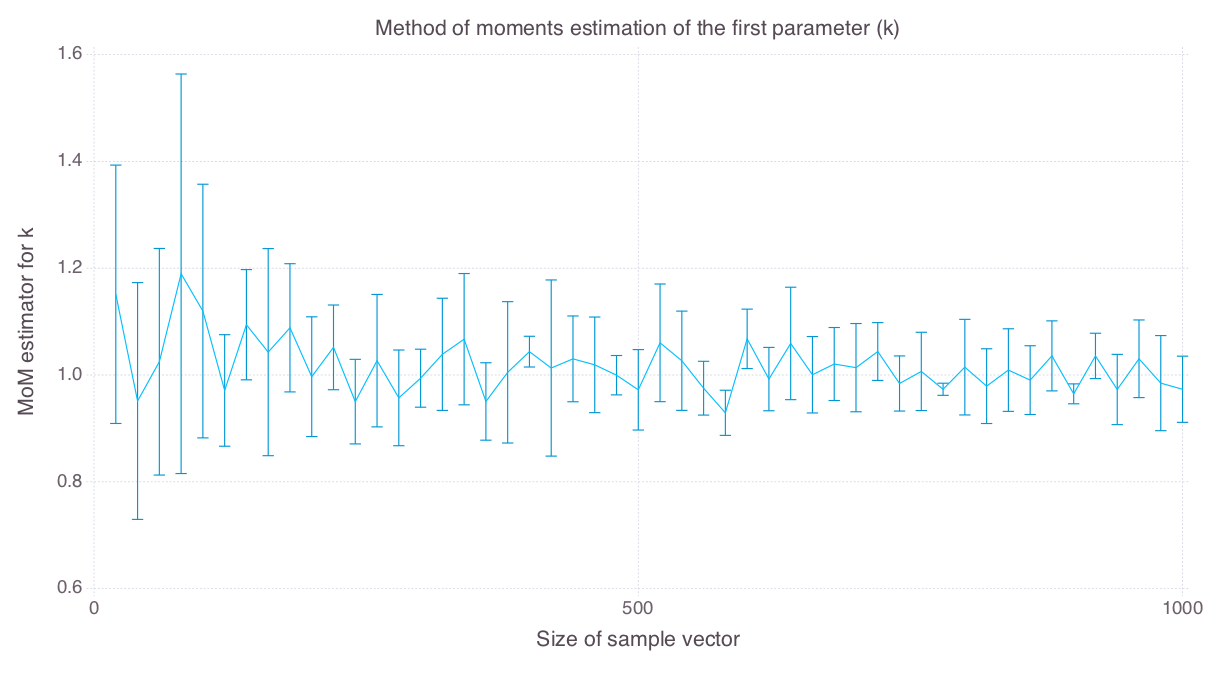
\includegraphics[width=\textwidth]{img/k_mom.png}
\end{figure}
\begin{figure}[H]
	\centering
	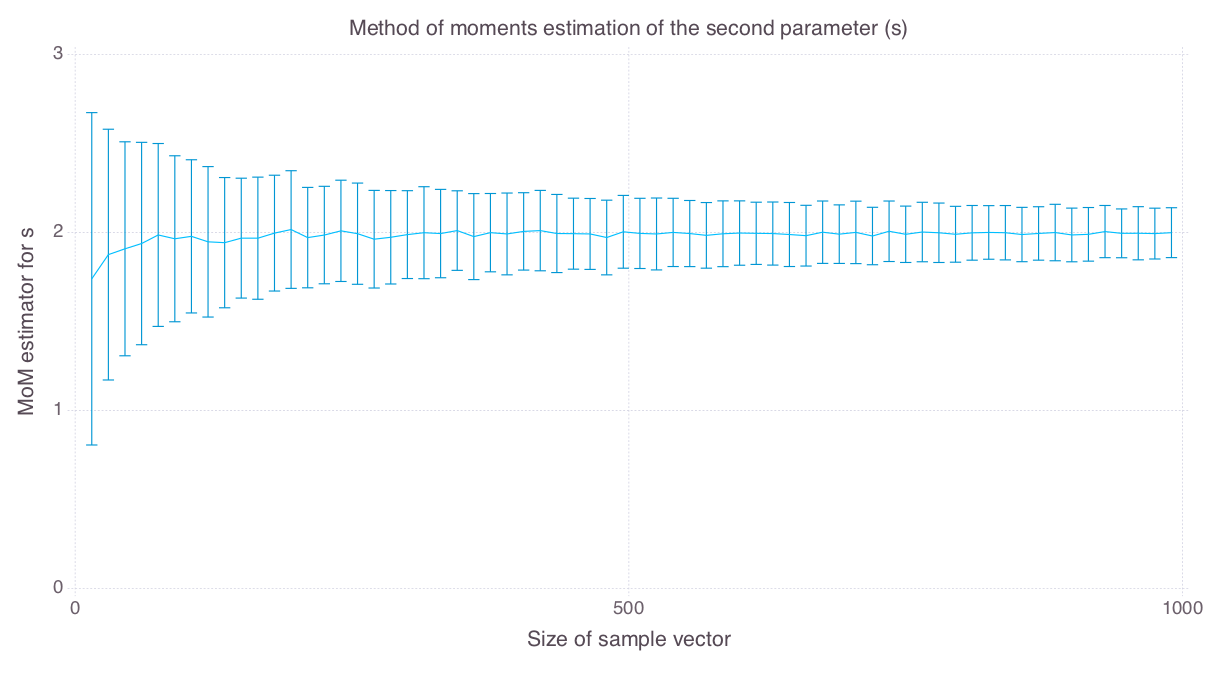
\includegraphics[width=\textwidth]{img/s_mom.png}
\end{figure}
\begin{figure}[H]
	\centering
	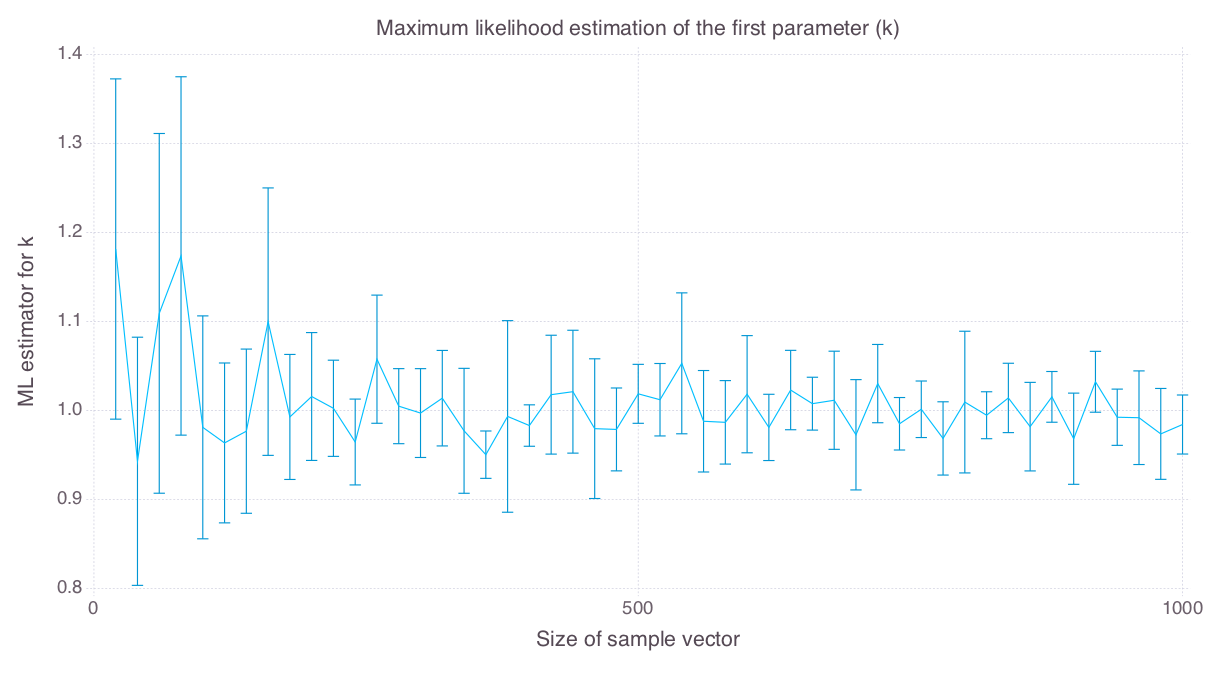
\includegraphics[width=\textwidth]{img/k_ml.png}
\end{figure}
\begin{figure}[H]
	\centering
	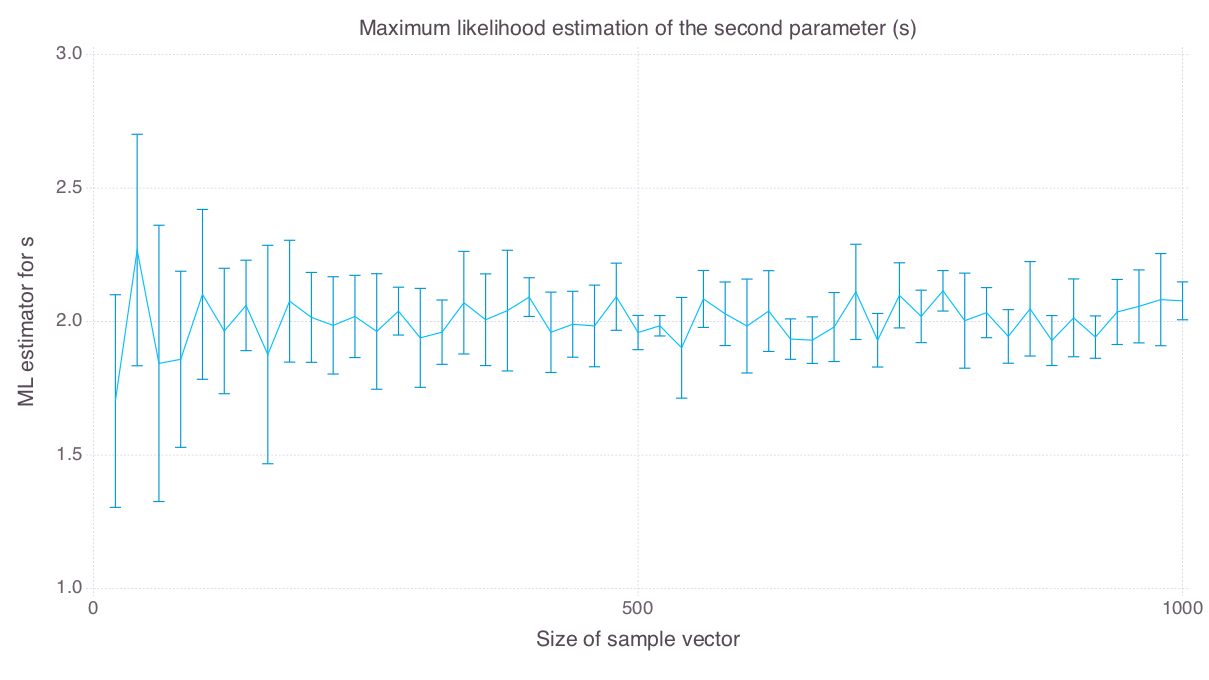
\includegraphics[width=\textwidth]{img/s_ml.png}
\end{figure}

\section{Fisher information matrix}
We can compute the Fisher information matrix. The entry $(i,j)$ of this matrix is given by equation \ref{information_matrix}. Since we have two estimators, this matrix is a $2\times 2$ matrix. Remember that
\begin{equation}
	\begin{aligned}
	lnf_Z(z,\theta) = h(z,\theta) & = ln\bigg( \frac{1}{\Gamma(k)s^k}x^{k-1}e^{-x/s} \bigg)\\
						   & = ln(x^{k-1}) + ln(e^{-x/s}) - ln(\Gamma(k)) - ln(s^k)\\
						   & = (k-1)ln(x) - \frac{x}{s} - ln(\Gamma(k)) - kln(s).
	\end{aligned}
\end{equation}
Therefore, before calculating the entries of the information matrix, we have to compute the partial derivatives before taking the expectation of it. Two examples of derivation are given in equations \ref{00} and \ref{11}. The procedure is similar for the other entries and the calculations can be found in Appendix \ref{fischer derivation}
\begin{equation}
	\begin{aligned}
	\frac{\partial h(z;\theta)}{\partial s} & = \frac{x}{s^2} - \frac{k}{s}
	\end{aligned}
\end{equation}
\begin{equation}
	\begin{aligned}
	\frac{\partial h(z;\theta)}{\partial k} & = ln(x) - \frac{1}{\Gamma(k)}\Gamma(k)\phi^{(0)}(k) - ln(s)\\
														  & = ln(x) - \phi^{(0)}(k) - ln(s).
	\end{aligned}
\end{equation}
\begin{equation}
	\begin{aligned}
	\frac{\partial^2h(z;\theta)}{\partial s^2} & = -\frac{x}{s^3}\cdot\frac{1}{2} + \frac{k}{s^2}.
	\end{aligned}
	\label{00}
\end{equation}
\begin{equation}
	\begin{aligned}
	\frac{\partial^2 h(z; \theta)}{\partial k^2} & = -\frac{d\phi^{(0)}(k)}{dk} = -\frac{d^2\Gamma(k)}{dk^2} = -\phi^{(1)}(k).
	\end{aligned}
	\label{11}
\end{equation}
Then, we take the expectation of these computed values.
\begin{equation}
	\begin{aligned}
	\fisher_{00} & = -\mathbb{E}\bigg\{ \frac{\partial^2 h(z;\theta)}{\partial s^2} \bigg\} = -\mathbb{E}\bigg\{ \frac{x}{s^2} - \frac{k}{s} \bigg\}\\
					   & = \frac{k}{s} - \frac{\mathbb{E}\{ x \}}{s^2} = \frac{k}{s} - \frac{ks}{s^2} = 0.
	\end{aligned}
\end{equation}
Finally, the Fisher information matrix is 
\[ \fisher(\theta) = \left( \begin{array}{cc}
	0              & \frac{1}{s} \\
	\frac{1}{s} & -\phi^{(1)}(k) \\
	 \end{array} \right)\] 
Then we have
\[ \fisher^{-1}(\theta) = \left( \begin{array}{cc}
	-\phi^{(1)}(k)s^2 & -s \\
	-s    & 0 \\
\end{array} \right) \] 
\section{Numerical proof}
\appendix
\section{\\Analytical derivations for d}
\subsection{Derivation of the Fisher information matrix coefficients}
\label{fischer derivation}
\begin{equation}
\begin{aligned}
\fisher_{01} & = -\mathbb{E}\bigg\{ \frac{\partial^2 h(z;\theta)}{\partial k\partial s} \bigg\}\\
& = -\mathbb{E}\bigg\{ -\frac{1}{s} \bigg\}\\
& = \frac{1}{s}.
\end{aligned}
\end{equation}
\begin{equation}
\begin{aligned}
\fisher_{10} & = \fisher_{01} = \frac{1}{s}.
\end{aligned}
\end{equation}
\begin{equation}
\begin{aligned}
\fisher_{11} & = -\mathbb{E}\bigg\{ \frac{\partial^2 h(z;\theta)}{\partial k^2} \bigg\}\\
& = -\mathbb{E}\bigg\{ \phi^{(1)}(k) \bigg\}\\
& = -\phi^{(1)}(k).
\end{aligned}
\end{equation}

Finally, the Fisher information matrix is 
\[ \fisher(\theta) = \left( \begin{array}{cc}
	0 & \frac{1}{s} \\
	\frac{1}{s} & -\phi^{(1)}(k) \\
	 \end{array} \right)\] 
\section{Numerical proof}

\appendix
\section{Omitted proofs}
\subsection{Proof of normality using the central limit theorem}
\label{app:banproof}
\begin{proof}
We want to prove that  \(\ell'(\theta_0)/\sqrt{N} \sim \mathcal{N}\big(0, \fisher(\theta_0)\big)\).
We simplify notation by writing \(\pdf(v_i)\) instead of \(\pdf_{V_i}(v_i; k, \theta)\)
and using Euler's notation for derivatives.
First, we show that the expected value of \(\ell'(\theta_0)/\sqrt{N}\) is zero.
\begin{align}
\expe{\frac{\ell'(\theta_0)}{\sqrt{N}}} &= \int_{-\infty}^{+\infty} \partial_{\theta_0} \left(\sum_{i=1}^N \frac{\ln \pdf(v_i)}{\sqrt{N}}\right) \pdf(v_i)\dif v_i\\
&= \frac{1}{\sqrt{N}} \sum_{i=1}^N \int_{-\infty}^{+\infty} \frac{\partial_\theta \pdf(v_i)}{\pdf(v_i)} \pdf(v_i)\dif v_i\\
&= \frac{1}{\sqrt{N}} \sum_{i=1}^N \int_{-\infty}^{+\infty} \frac{\partial_\theta \pdf(v_i)}{\pdf(v_i)} \pdf(v_i) \dif v_i\\
&= \frac{1}{\sqrt{N}} \sum_{i=1}^N \int_{-\infty}^{+\infty} \partial_\theta \pdf(v_i) \dif v_i\\
&= \frac{1}{\sqrt{N}} \sum_{i=1}^N \partial_\theta \int_{-\infty}^{+\infty} \pdf(v_i) \dif v_i\\
&= 0\,.
\end{align}

Next, we compute the variance of \(\ell'(\theta_0)/\sqrt{N}\).
First, we compute (for \(i = 1, \ldots, N\))
\begin{align}
\expe{\big(\partial_{\theta_0} \ln \pdf(v_i)\big)^2} &= \int_{-\infty}^{+\infty} \partial_{\theta_0} \ln \pdf(v_i) \frac{\partial_{\theta_0} \pdf(v_i)}{\pdf(v_i)} \pdf(v_i)\dif v_i\\
&= \int_{-\infty}^{+\infty} \partial_{\theta_0} \ln \pdf(v_i) \partial_{\theta_0} \pdf(v_i) \dif v_i\,.
\intertext{Using the product rule, we can then find}
&= \begin{multlined}[t]
- \int_{-\infty}^{+\infty} \partial_{\theta_0 \theta_0} \ln \pdf(v_i) \pdf(v_i) \dif v_i \\
+ \int_{-\infty}^{+\infty} \partial_{\theta_0} \big(\partial_{\theta_0} \ln \pdf(v_i) \pdf(v_i)\big) \dif v_i\,.
\end{multlined}\\
&= - \expe{\partial_{\theta_0 \theta_0 } \ln \pdf(v_i)} + \partial_{\theta_0} \int_{-\infty}^{\infty} \frac{\partial_{\theta_0} \pdf(v_i)}{\pdf(v_i)} \pdf(v_i) \dif v_i\\
&= \fisher(\theta)\,,
\end{align}
where the last expression can be shown to be zero by a similar argument as the one used above for the expected value.
Knowing this, one easily finds
\begin{equation}
\var{\frac{\ell'(\theta_0)}{\sqrt{N}}} = \frac{1}{N} \var{\sum_{i=1}^N \partial_{\theta_0} \ln \pdf(v_i)} = \fisher(\theta_0)\,,
\end{equation}
since the random variables are i.i.d..
Using the Lindeberg--Lévy CLT, we thus have
\begin{equation}
\frac{\ell'(\theta_0)}{\sqrt{N}} \sim \mathcal{N}(0, \fisher(\theta_0))\,.\qedhere
\end{equation}

\end{proof}
\bibliography{report-linma1731-project}
\bibliographystyle{aomalpha}

\end{document}
\endinput
